\mychapter{3}{Input variable analysis}
\label{sec:unchapitre}

A large set of variables is available from CMS data but MVA training can be time consumming and the "curse of
dimensionality" \footnote{Curse of dimensionality refers to problems that commonly arise when analyzing high-dimensionality data.
Increasing dimensionality lead to an increase of volume and so tends to scatter data points.} forces us to select only a few of them based on two main criteria :
\begin{description}
    \item [Background vs Signal discrimination :] Variables with most differences of shape for background and signal will be picked.
    \item [Low correlation between variables :] Needed in order to reduce redundancy of input data and thus will permit
    to reduce MVA complexity (for example number of hidden neurons in ANN).
\end{description}

The MVA will be trained with MC simulation for the signal sample and with the real data for the background sample.
In order to do that we need to perform a data-driven background estimation using a low-correlated variable for a
sideband definition.

\section{Background vs Signal discrimination}

It is necessary to pick the smallest set of input variable for the MVA. This selection is done by looking at variable
shape for background and signal data from MC simulation.\\
Then a cross-check of the variables shape has to be done between Data and MC.\\
Here an example of MC simulation and data comparison for \emph{neutral hadron isolation} variable.(fig.
\ref{NHiso_photon_dataVsMCbg}) \\

\begin{figure}[h!]
  \centering
  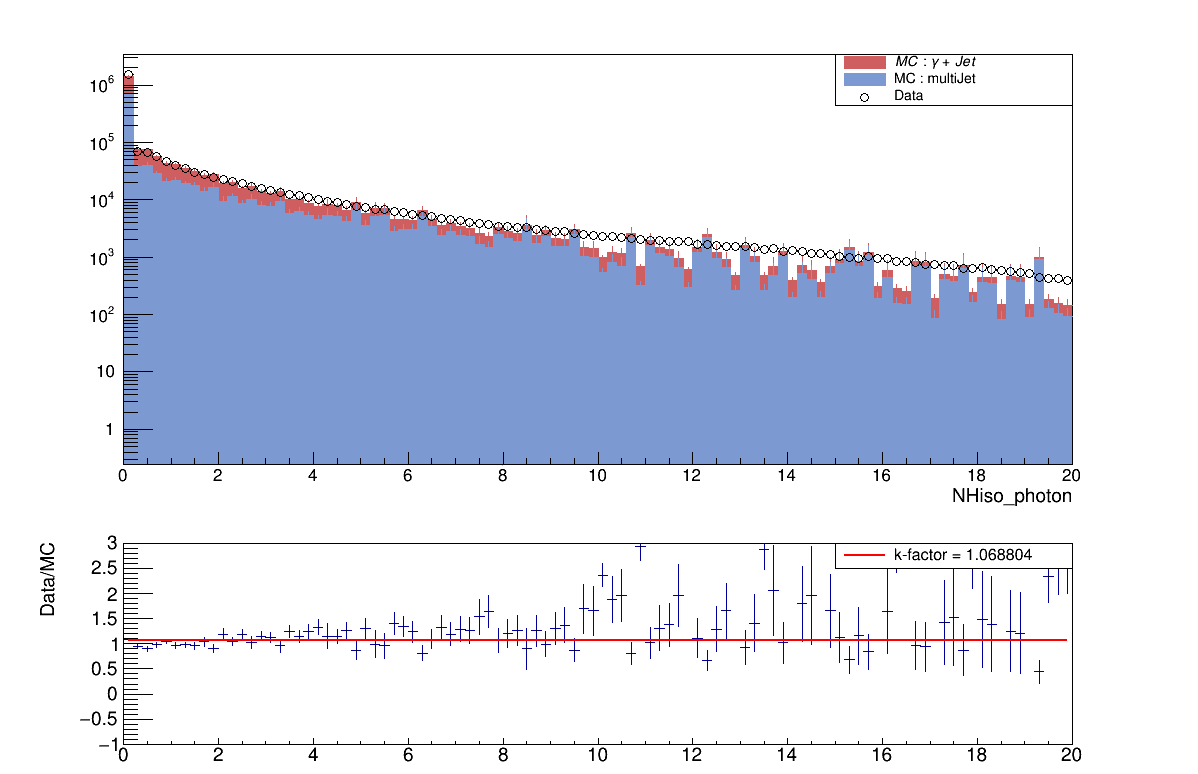
\includegraphics[width=0.8\textwidth]{NHiso_photon}\\[1cm]
  \caption{Neutral hadron isolation for background and signal MC}
  \label{NHiso_photon_dataVsMCbg}
\end{figure}

\section{Variable correlations}

Training data needed-quantity increases with network complexity, so correlation between variables must be avoided in
order to get the minimum redundancy.\\
One of these variables has to be used for the data-driven background estimation, by looking at the correlation matrix
(fig. \ref{corrMatrix_bgMC}) we can see that \emph{charged hadron isolation} is one good candidate and so will be used next for the sideband
definition.//

\begin{figure}[ht!]
  \centering
  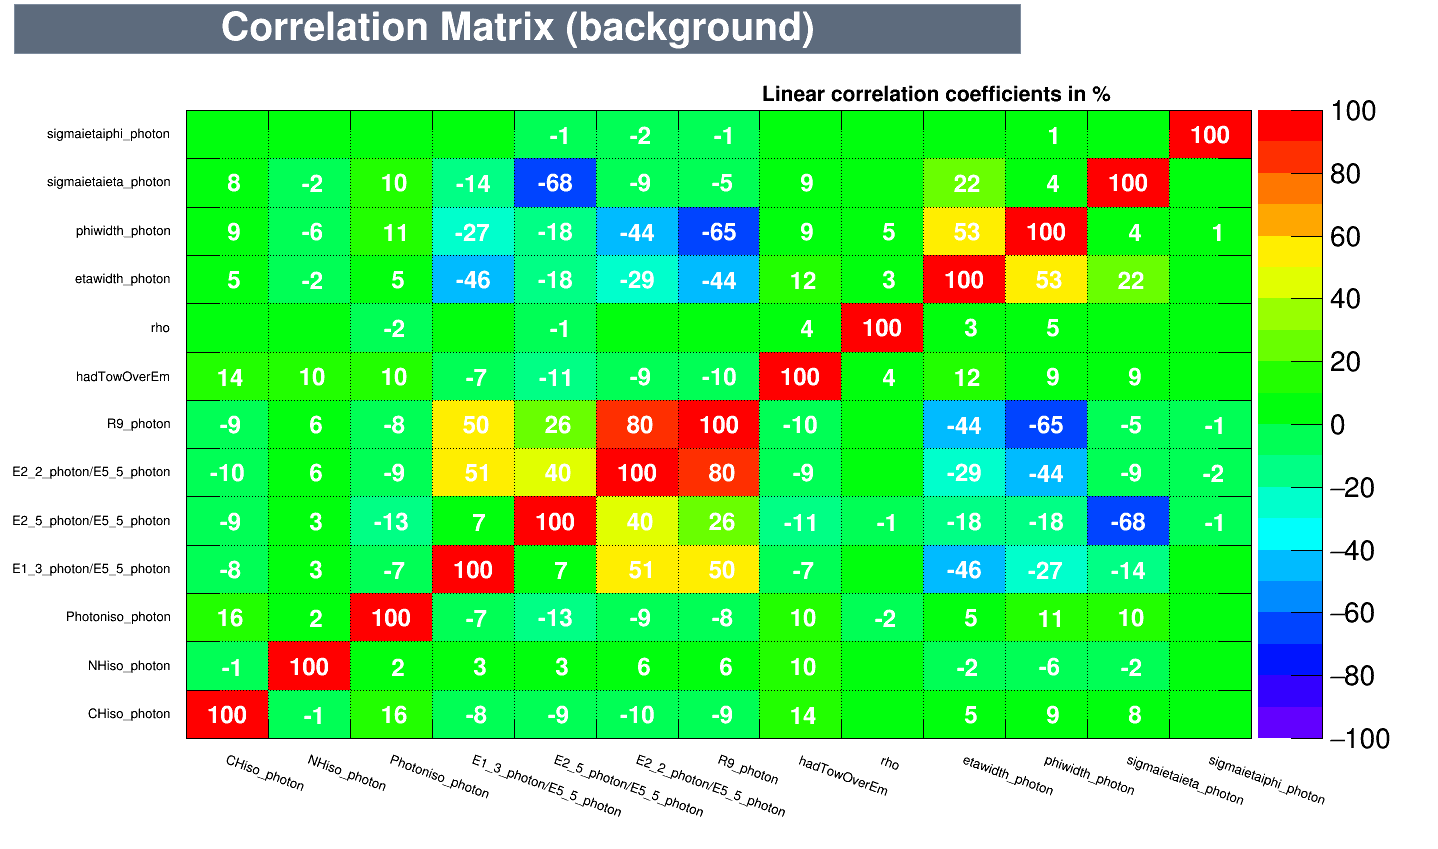
\includegraphics[width=0.8\textwidth]{corrMatrix_bgMC}\\[1cm]
  \caption{Correlation matrix for background MC}
  \label{corrMatrix_bgMC}
\end{figure}

\section{Data driven background estimation}

MVA will be performed with real data for the background, thereby a sideband (background enriched region in the data sample) has to be defined on a low-correlated
variable (fig. \ref{sideband}) that won't be used in the MVA. A cut has been applied on \emph{charged hadron isolation}\\ in order to get the best ratio of background purity over number of events.
\begin{description}
	\item [Sideband definition]
	\begin{description}
    	\item 2.325 < \emph{Charge hadron isolation} < 15.
    	\item Background purity = 95.00 \%
		\item Number of events = $7.59*10^5$
	\end{description}
\end{description}

Then a signal enriched region has been defined on the same variable, this cut will be applied on the signal data sample.
\begin{description}
	\item [Signal region definition]
	\begin{description}
    	\item \emph{Charge hadron isolation} < 2.
    	\item Signal purity = ?? \%
		\item Number of events = ??
	\end{description}
\end{description}

\begin{figure}[ht!]
  \centering
  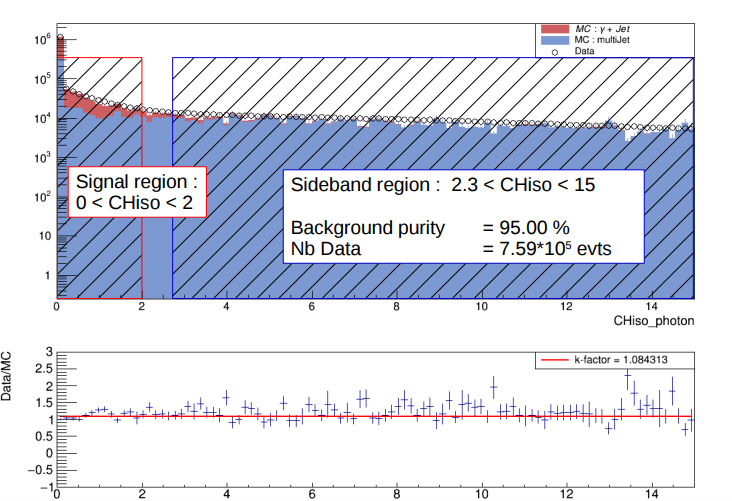
\includegraphics[width=0.8\textwidth]{sideband}\\[1cm]
  \caption{Charged hadron isolation for background and signal MC (histograms), signal region (red shaded area) and
  sideband (blue shaded area).}
  \label{sideband}
\end{figure}

For cross-checking, we compare variables shape for background MC and DATA in the sideband region.
Here you can see for example a comparison between \emph{neutral hadron isolation} for data in the sideband region and background Monte-Carlo.(fig. \ref{MCbg_all_NHiso_photon}) 

\begin{figure}[h!]
  \centering
  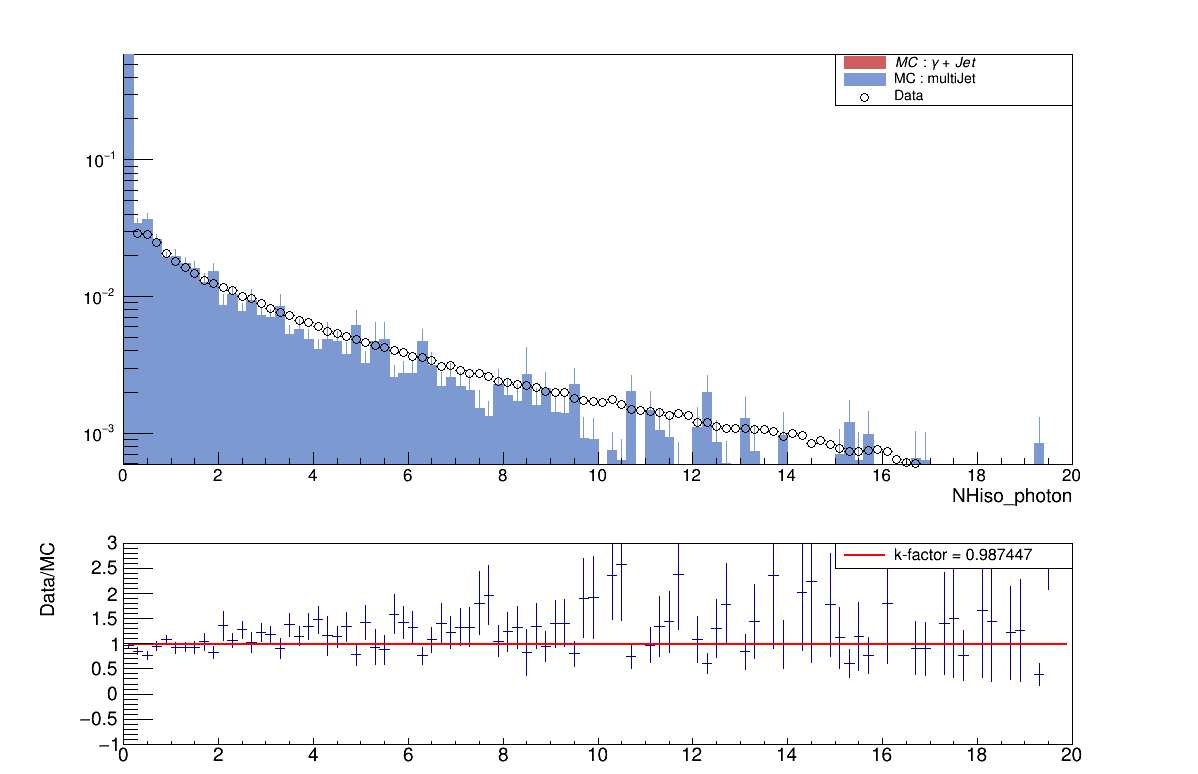
\includegraphics[width=0.8\textwidth]{MCbg_all_NHiso_photon}\\[1cm]
  \caption{Neutral hadron isolation for background MC and DATA in the sideband region}
  \label{MCbg_all_NHiso_photon}
\end{figure}

%%% Local Variables: 
%%% mode: latex
%%% TeX-master: "isae-report-template"
%%% End: 
